\subsection{1. Giao diện sản phẩm}

\indent\indent Hệ thống \textit{SybilSignal} được hiện thực hóa dưới dạng một bảng điều khiển tương tác, hỗ trợ song ngữ (Anh - Việt) nhằm tối ưu hóa khả năng tiếp cận dữ liệu Web3 quốc tế. Giao diện được thiết kế phân cấp thành hai phân hệ chiến lược: Xác minh thực thể và Khám phá mạng lưới.\vspace{0.3cm}

\textbf{1.1. Phân hệ xác minh thực thể}\vspace{0.2cm}

Phân hệ này phục vụ mục đích kiểm định chuyên sâu và giải thích hành vi cho từng tài khoản cụ thể thông qua mã định danh hồ sơ.\vspace{0.3cm}

\textbf{Quy trình xác minh:} Người dùng thực hiện nhập \texttt{profile\_id} vào hệ thống để kích hoạt quy trình truy vấn đặc trưng và suy luận nhãn dựa trên mô hình GNN đã được huấn luyện.

\begin{figure}[H]
    \centering
    \fbox{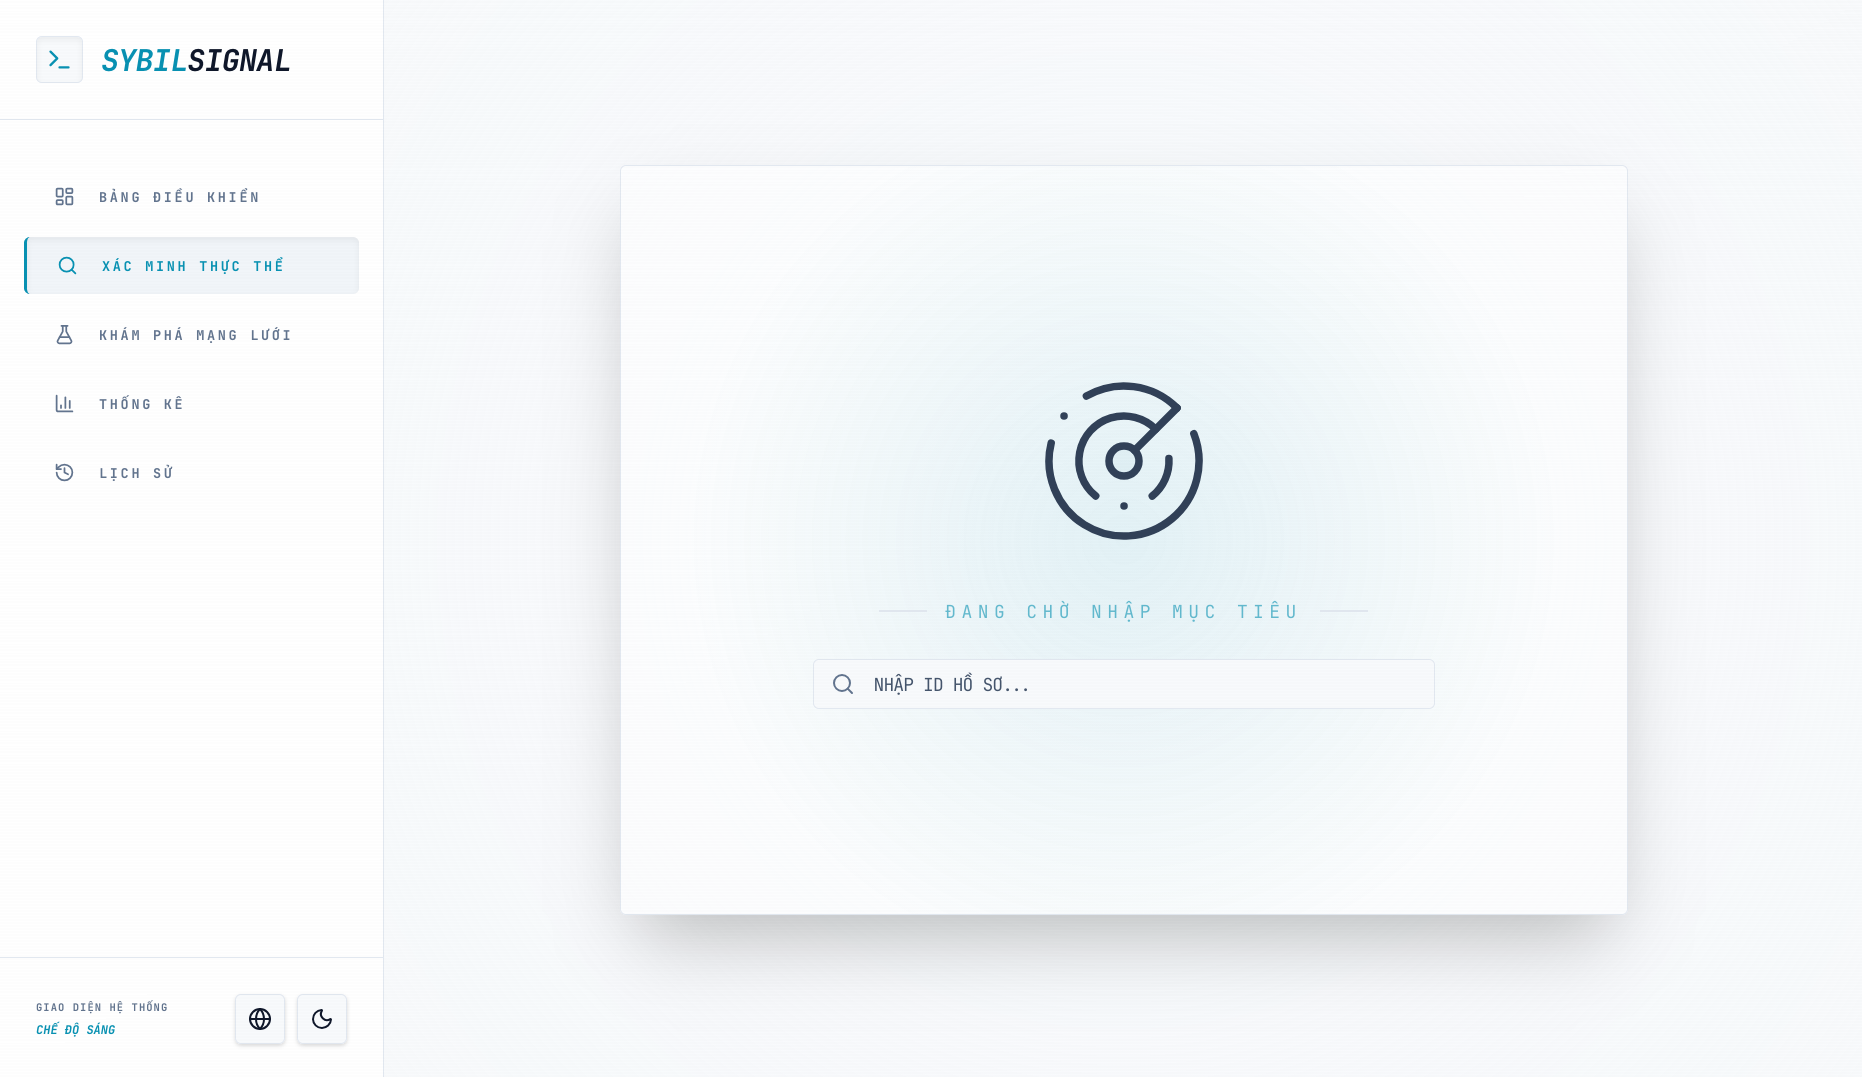
\includegraphics[width=\linewidth]{images/part-02/chap-03/sec-01/InspectorInputSearch.png}}
    \vspace{0.1cm}
    \caption{Giao diện nhập mã định danh trong phân hệ Xác minh thực thể}
    \label{fig:InspectorInputSearch}
\end{figure}

\textbf{Trực quan hóa đồ thị cục bộ (Ego-graph):} Hệ thống hiển thị nhãn dự đoán kèm theo cấu trúc đồ thị cục bộ bao quanh nút mục tiêu. Giao diện cung cấp bộ công cụ tương tác mạnh mẽ để bóc tách các mối quan hệ:
\begin{itemize}[label={--}, itemsep=1pt]
    \item \textbf{Tùy chỉnh độ sâu quan hệ:} Hỗ trợ lựa chọn hiển thị láng giềng bậc 1 hoặc bậc 2 để mở rộng phạm vi phân tích cấu trúc mạng lưới.
    \item \textbf{Tối ưu hóa hiển thị:} Cung cấp chức năng ẩn/hiện các cạnh không liên quan trực tiếp và gộp các cạnh giữa hai nút để giảm nhiễu trực quan.
    \item \textbf{Trực quan hệ số chú ý:} Hệ thống hiển thị trọng số chú ý (\textit{GAT Attention Weight}) trực tiếp trên từng cạnh, cho thấy mức độ quan trọng của từng láng giềng đóng góp vào quyết định phân loại của mô hình.
\end{itemize}

\begin{figure}[H]
    \centering
    \fbox{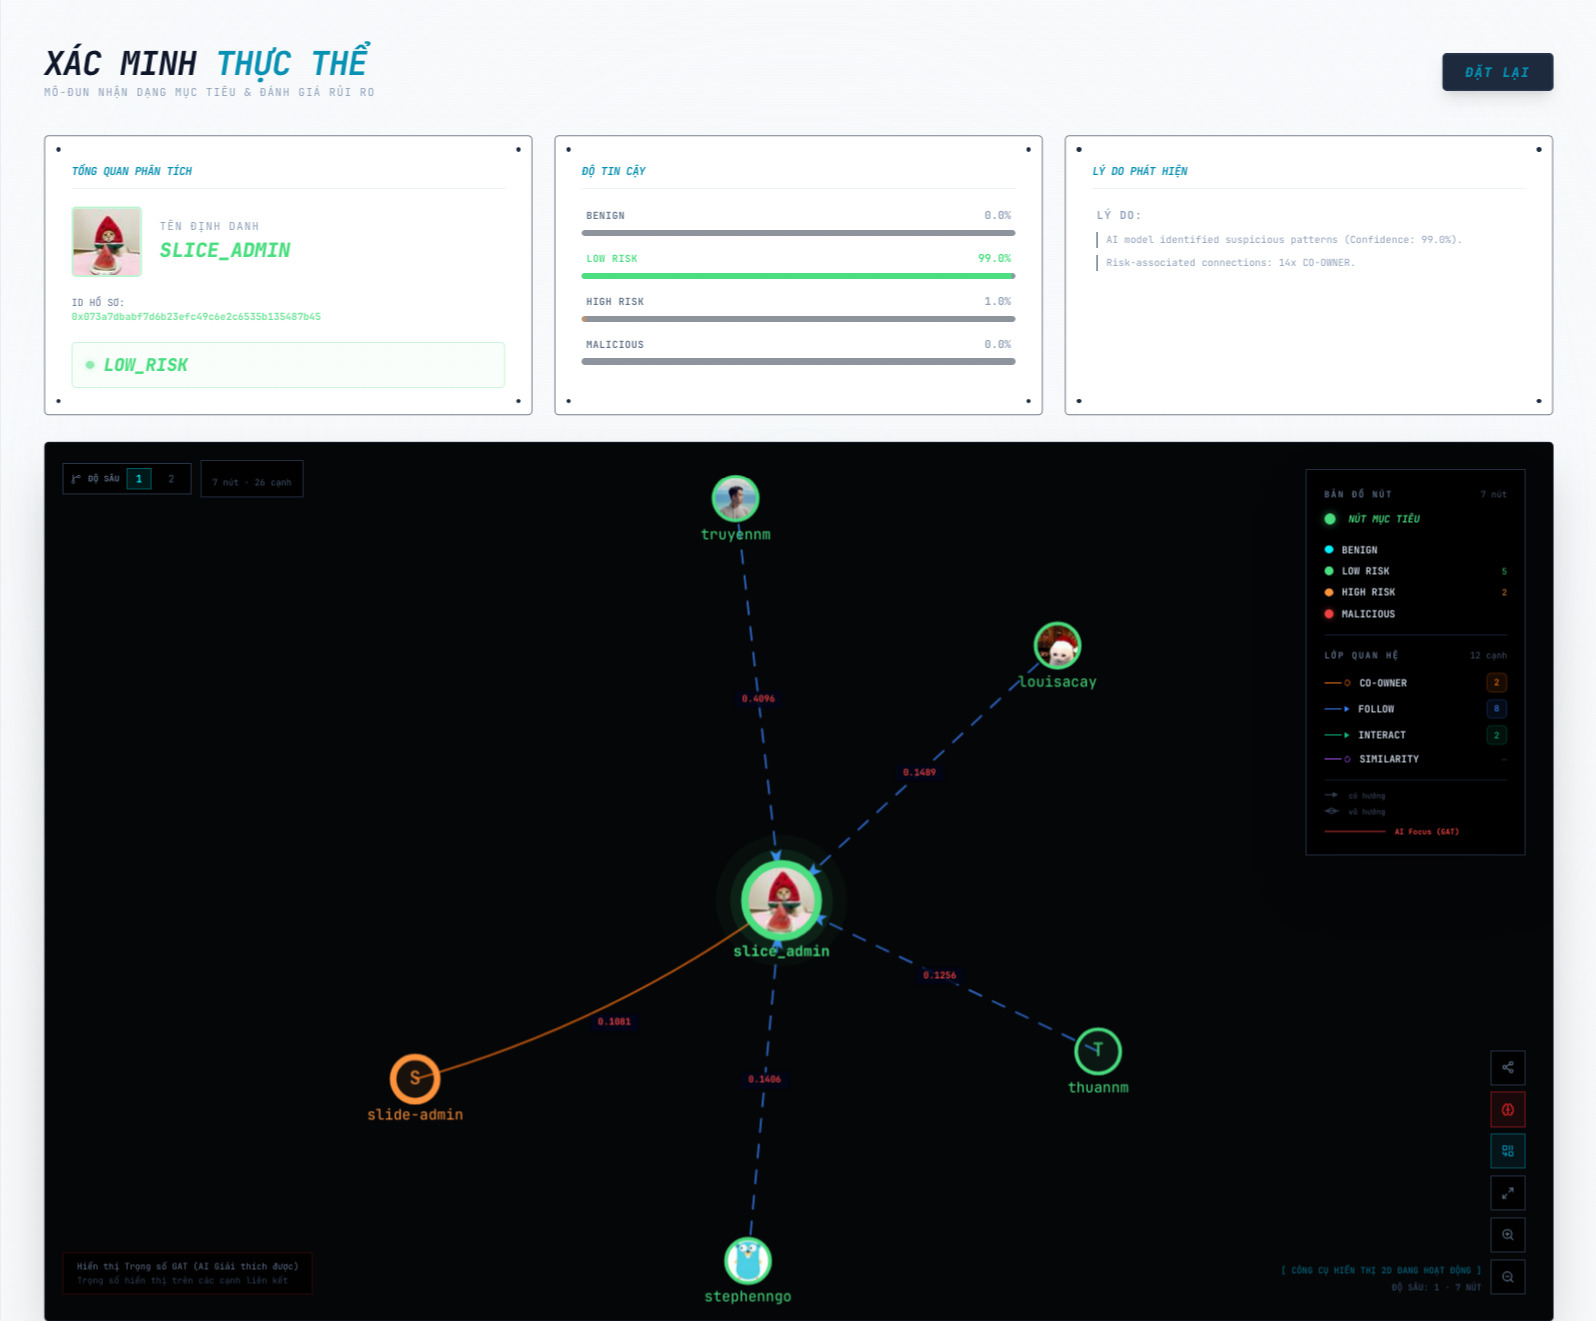
\includegraphics[width=\linewidth]{images/part-02/chap-03/sec-01/InspectorResultGraph.png}}
    \vspace{0.1cm}
    \caption{Giao diện hiển thị kết quả xác minh và đồ thị tương tác cục bộ}
    \label{fig:InspectorResultGraph}
\end{figure}

\textbf{Tính giải thích thông qua dữ liệu tham chiếu:} Điểm vượt trội của phân hệ này là khả năng giải thích. Khi tương tác với các nút, hệ thống truy xuất thông tin chi tiết từ tập dữ liệu tham chiếu (kết quả quy trình GAE + KMeans). Việc đối chiếu giữa kết quả dự đoán hiện tại và lý do gán nhãn lịch sử giúp chuyên gia hiểu rõ "mô thức" hành vi mà mô hình đang sử dụng để nhận diện Sybil.\vspace{0.3cm}

\textbf{1.2. Phân hệ khám phá mạng lưới}\vspace{0.2cm}

Phân hệ này cho phép phân tích các cụm dữ liệu diện rộng theo phạm vi thời gian và cấu hình tham số linh hoạt để nhận diện các mô thức bầy đàn. Sau quá trình xử lý và gom cụm bởi AI, kết quả được hệ thống trực quan hóa thành một đồ thị liên kết đa tầng với độ tương tác cao.\vspace{0.3cm}

\textbf{Cấu hình tham số và siêu tham số:} Người dùng có thể thiết lập các ràng buộc về thời gian và giới hạn quy mô nút. Đặc biệt, giao diện hỗ trợ điều chỉnh các siêu tham số huấn luyện như số vòng lặp (\textit{Epochs}), tốc độ học (\textit{Learning Rate}) và ngưỡng dừng sớm (\textit{Patience}).

\begin{figure}[H]
    \centering
    \fbox{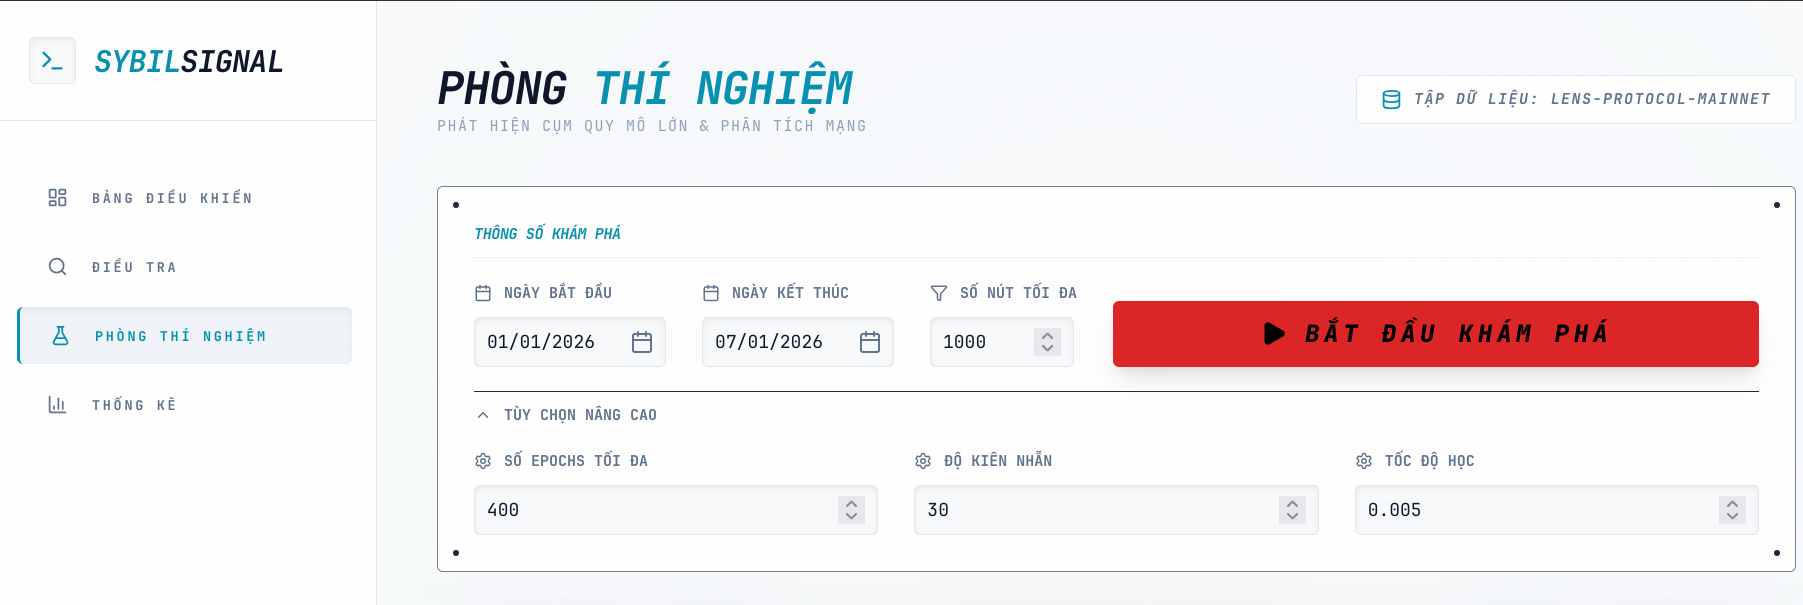
\includegraphics[width=\linewidth]{images/part-02/chap-03/sec-01/DiscoveryInputConfig.png}}
    \vspace{0.1cm}
    \caption{Giao diện nhập phạm vi dữ liệu và siêu tham số khám phá}
    \label{fig:DiscoveryInputConfig}
\end{figure}

\textbf{Trực quan hóa mạng lưới tổng thể:} Ở góc nhìn toàn cảnh, hệ thống hiển thị toàn bộ các nút trong phạm vi truy vấn (Hình \ref{fig:DiscoveryGlobalView}). Người dùng có thể quan sát nhanh sự phân bổ của các cụm hành vi khác nhau được mã hóa bằng màu sắc. Đồ thị giúp nhận diện ngay lập tức sự khác biệt về mặt cấu trúc: các mạng lưới Sybil thường co cụm thành các nhóm nhỏ khép kín và tách biệt, trong khi cộng đồng người dùng thật tạo thành mạng lưới liên kết hữu cơ, phân tán và rộng lớn hơn.

\begin{figure}[H]
    \centering
    \fbox{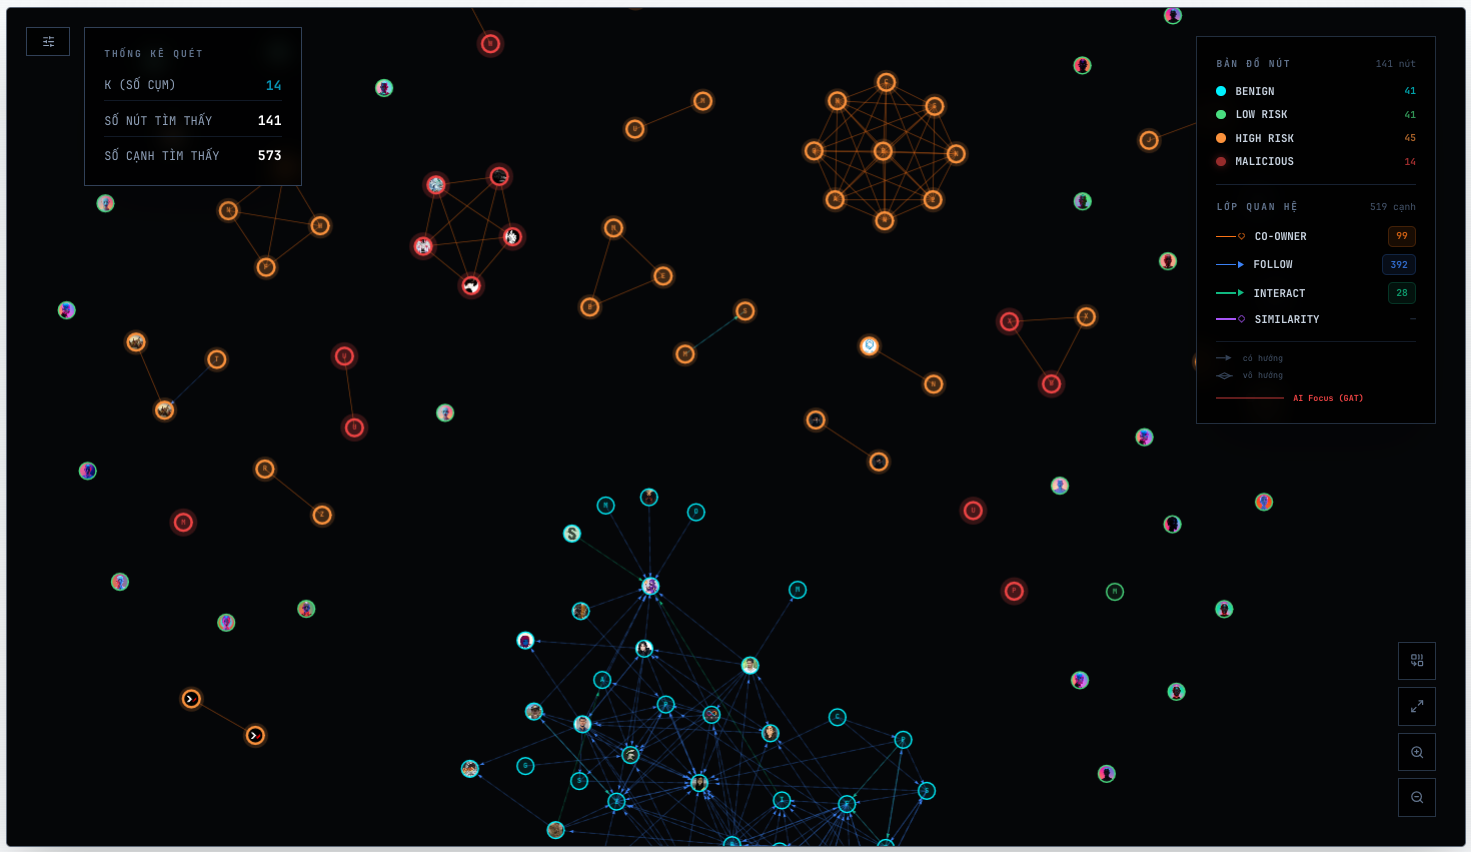
\includegraphics[width=\linewidth]{images/part-02/chap-03/sec-01/DiscoveryGlobalView.png}}
    \vspace{0.1cm}
    \caption{Giao diện trực quan hóa đồ thị mạng lưới diện rộng và phân bổ các cụm}
    \label{fig:DiscoveryGlobalView}
\end{figure}

\textbf{Khảo sát chi tiết cụm người dùng hợp lệ:} Khi phóng to vào cụm hành vi (Hình \ref{fig:DiscoveryBenignCluster}), hệ thống cung cấp giao diện phân tích vi mô cho một nhóm người dùng thật.

\begin{figure}[H]
    \centering
    \fbox{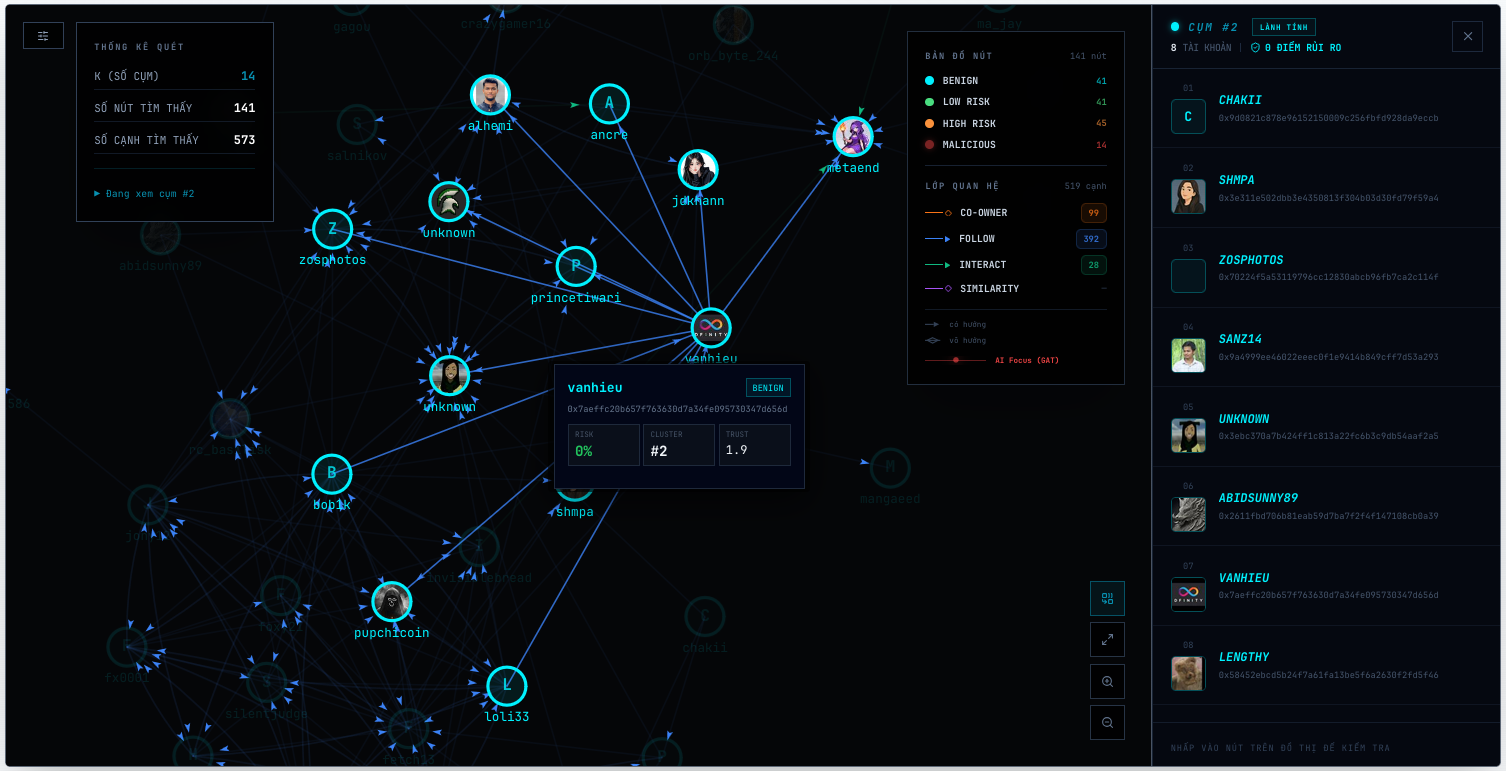
\includegraphics[width=\linewidth]{images/part-02/chap-03/sec-01/DiscoveryBenignCluster.png}}
    \vspace{0.1cm}
    \caption{Giao diện chi tiết phân tích cụm người dùng thật}
    \label{fig:DiscoveryBenignCluster}
\end{figure}

\textbf{Nhận diện và phân tích cụm Sybil:} Ngược lại, khi chuyển sang khảo sát cụm rủi ro cao (Hình \ref{fig:DiscoverySybilCluster}), các mô thức bầy đàn lộ diện rõ nét.

\begin{figure}[H]
    \centering
    \fbox{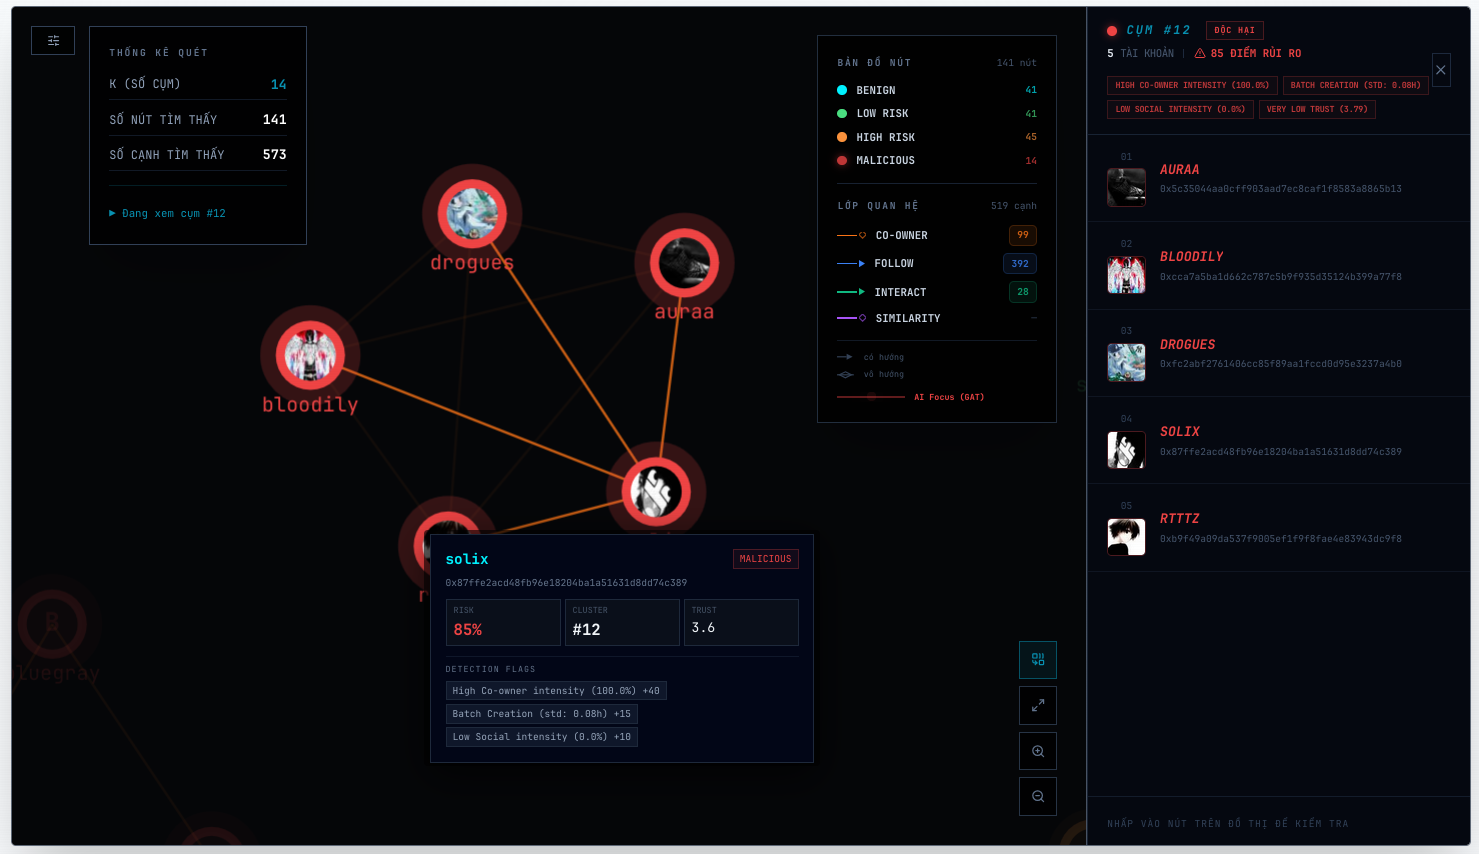
\includegraphics[width=\linewidth]{images/part-02/chap-03/sec-01/DiscoverySybilCluster.png}}
    \vspace{0.1cm}
    \caption{Giao diện phát hiện và phân tích cảnh báo cụm tài khoản Sybil}
    \label{fig:DiscoverySybilCluster}
\end{figure}